\let\negmedspace\undefined
\let\negthickspace\undefined
\documentclass[journal,12pt,onecolumn]{IEEEtran}
\usepackage{cite}
\usepackage{amsmath,amssymb,amsfonts,amsthm}
\usepackage{algorithmic}
\usepackage{graphicx}
\graphicspath{{./figs/}}
\usepackage{textcomp}
\usepackage{xcolor}
\usepackage{txfonts}
\usepackage{listings}
\usepackage{enumitem}
\usepackage{mathtools}
\usepackage{gensymb}
\usepackage{comment}
\usepackage{caption}
\usepackage[breaklinks=true]{hyperref}
\usepackage{tkz-euclide} 
\usepackage{listings}
\usepackage{gvv}                                        
%\def\inputGnumericTable{}                                 
\usepackage[latin1]{inputenc}     
\usepackage{xparse}
\usepackage{color}                                            
\usepackage{array}
\usepackage{longtable}                                       
\usepackage{calc}                                             
\usepackage{multirow}
\usepackage{multicol}
\usepackage{hhline}                                           
\usepackage{ifthen}                                           
\usepackage{lscape}
\usepackage{tabularx}
\usepackage{array}
\usepackage{float}
\newtheorem{theorem}{Theorem}[section]
\newtheorem{problem}{Problem}
\newtheorem{proposition}{Proposition}[section]
\newtheorem{lemma}{Lemma}[section]
\newtheorem{corollary}[theorem]{Corollary}
\newtheorem{example}{Example}[section]
\newtheorem{definition}[problem]{Definition}
\newcommand{\BEQA}{\begin{eqnarray}}
\newcommand{\EEQA}{\end{eqnarray}}
\newcommand{\define}{\stackrel{\triangle}{=}}
\theoremstyle{remark}
\newtheorem{rem}{Remark}

\begin{document}
\title{Assignment 2 : GATE PE 2022}
\author{ee25btech11056 - Suraj.N}
\maketitle
\renewcommand{\thefigure}{\theenumi}
\renewcommand{\thetable}{\theenumi}

\begin{enumerate}

\item After playing \_\_\_\_\_\_\_\_\_ hours of tennis, I am feeling \_\_\_\_\_\_\_\_ tired to walk back. 

\hfill{\brak{\text{GATE PE 2022}}}

\begin{enumerate}
\begin{multicols}{4}
\item too/too
\item too/two
\item two/two
\item two/too
\end{multicols}
\end{enumerate}

\item The average of the monthly salaries of M, N and S is  rupees $4000$. The average of the monthly salaries of N, S and P is rupees $5000$. The monthly salary of P is rupees $6000$. What is the monthly salary of M as a percentage of the monthly salary of P?

\hfill{\brak{\text{GATE PE 2022}}}

\begin{enumerate}
\begin{multicols}{4}
\item $50\%$
\item $75\%$
\item $100\%$
\item $125\%$
\end{multicols}
\end{enumerate}

\item A person travelled $80$ km in $6$ hours. If the person travelled the first part with a uniform speed of $10$ kmph and the remaining part with a uniform speed of $18$ kmph. What percentage of the total distance is travelled at a uniform speed of $10$ kmph?

\hfill{\brak{\text{GATE PE 2022}}}

\begin{enumerate}
\begin{multicols}{4}
\item 28.25
\item 37.25
\item 43.75
\item 50.00
\end{multicols}
\end{enumerate}

\item Four girls P, Q, R and S are studying languages in a University. P is learning French and Dutch. Q is learning Chinese and Japanese. R is learning Spanish and French. S is learning Dutch and Japanese.  

Given that: French is easier than Dutch; Chinese is harder than Japanese; Dutch is easier than Japanese, and Spanish is easier than French.  

Based on the above information, which girl is learning the most difficult pair of languages?

\hfill{\brak{\text{GATE PE 2022}}}

\begin{enumerate}
\begin{multicols}{4}
\item P
\item Q
\item R
\item S
\end{multicols}
\end{enumerate}
 
\pagebreak

\item A block with a trapezoidal cross-section is placed over a block with rectangular
cross section as shown below.\\
Which one of the following is the correct drawing of the view of the 3D object
as viewed in the direction indicated by an arrow in the above figure?

\hfill{\brak{\text{GATE PE 2022}}}

\begin{figure}[h!]
  \centering
  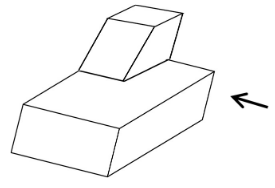
\includegraphics[width=0.3\columnwidth]{figs/fig1.png} 
   \caption*{}
  \label{fig:Q5}
\end{figure}

\begin{enumerate}
\begin{multicols}{4}
\item 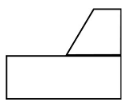
\includegraphics[width=2cm]{figs/fig2.png} 
\item 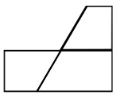
\includegraphics[width=2cm]{figs/fig3.png}
\item 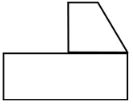
\includegraphics[width=2cm]{figs/fig4.png}
\item 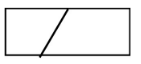
\includegraphics[width=2cm]{figs/fig5.png}
\end{multicols}
\end{enumerate}

\item Humans are naturally compassionate and honest. In a study using strategically placed wallets that appear "lost", it was found that wallets with money are more likely to be returned than wallets without money. Similarly, wallets that had a key and money are more likely to be returned than wallets with the same amount of money alone. This suggests that the primary reason for this behavior is compassion and empathy.  

Which one of the following is the CORRECT logical inference based on the information inthe above passage?

\hfill{\brak{\text{GATE PE 2022}}}

\begin{enumerate}
\item Wallets with a key are more likely to be returned because people do not care about money
\item Wallets with a key are more likely to be returned because people relate to suffering of others
\item Wallets used in experiments are more likely to be returned than wallets that are really lost
\item Money is always more important than keys
\end{enumerate}

\item A rhombus is formed by joining the midpoints of the sides of a unit square. What is the diameter of the largest circle that can be inscribed within the rhombus?

\hfill{\brak{\text{GATE PE 2022}}}

\begin{enumerate}
\begin{multicols}{4}
\item $\frac{1}{\sqrt{2}}$
\item $\frac{1}{2\sqrt{2}}$
\item $\sqrt{2}$
\item $2\sqrt{2}$
\end{multicols}
\end{enumerate}

\item An equilateral triangle, a square and a circle have equal areas. What is the ratio of the perimeters of the equilateral triangle to square to circle?

\hfill{\brak{\text{GATE PE 2022}}}

\begin{enumerate}
\begin{multicols}{4}
\item $3\sqrt{3} : 2 : \sqrt{\pi}$
\item $3 \sqrt{3} : 2 : \sqrt{\pi}$
\item $3 \sqrt{3} : 4 : 2\sqrt{\pi}$
\item $3 \sqrt{3} : 2 : 2\sqrt{\pi}$
\end{multicols}
\end{enumerate}

\pagebreak

\item Given below are three conclusions drawn based on the following three statements.

\begin{enumerate}
\item All teachers are professors.
\item No professor is a male.  
\item Some males are engineers. 
\end{enumerate}

\begin{enumerate}
\item No engineer is a professor.
\item Some engineers are professors.  
\item No male is a teacher.  
\end{enumerate}

Which one of the following options can be logically inferred?

\hfill{\brak{\text{GATE PE 2022}}}

\begin{enumerate}
\item Only conclusion III is correct
\item Only conclusion I and conclusion II are correct
\item Only conclusion II and conclusion III are correct
\item Only conclusion I and conclusion III are correct
\end{enumerate}

\item In a $12$-hour clock that runs correctly, how many times do the second, minute, and hour hands of the clock coincide, in a 12-hour duration from 3 PM in a day to 3 AM the next day?

\hfill{\brak{\text{GATE PE 2022}}}

\begin{enumerate}
\begin{multicols}{4}
\item 11
\item 12
\item 144
\item 2
\end{multicols}
\end{enumerate}

\item The value of  
\begin{align*}
\lim_{x \to 0} \frac{\ln(1+x)}{x}
\end{align*}
is

\hfill{\brak{\text{GATE PE 2022}}}

\begin{enumerate}
\begin{multicols}{4}
\item $e$
\item $1$
\item $0$
\item $\frac{1}{e}$
\end{multicols}
\end{enumerate}

\item The following second order ordinary differential equation has the boundary conditions: $y(0) = 0$, and $y(1) = 1$.  
\begin{align*}
\frac{d y}{d x} + \frac{d y}{d x} = 5 y
\end{align*}
The type of above boundary conditions is

\hfill{\brak{\text{GATE PE 2022}}}

\begin{enumerate}
\begin{multicols}{4}
\item Neumann
\item Dirichlet
\item Cauchy
\item Robin
\end{multicols}
\end{enumerate}

\item Let $\vec{F}(x,y) = e^{\sin x} \hat{i} + x \hat{j}$ for $(x, y) \in \mathbb{R}^2$. If $C$ is the circle $x^2 + y^2 = 4$ oriented anticlockwise, then

\begin{align*}
\oint_C \vec{F} \cdot d\vec{R}
\end{align*}
equals

\hfill{\brak{\text{GATE PE 2022}}}

\begin{enumerate}
\begin{multicols}{4}
\item $4\pi$
\item $6\pi$
\item $7\pi$
\item $8\pi$
\end{multicols}
\end{enumerate}

\pagebreak

\item The general equation for the production rate decline can be expressed as

\begin{align*}
\frac{1}{q} \frac{dq}{dt} = -b q
\end{align*}

where $b$ and $d$ are empirical constants, and $q$ is the production rate.  

Match the value of $d$ (Group 1) with the appropriate decline curves (Group 2).  

\begin{tabular}{|c|c|}
\hline
\textbf{Group 1} & \textbf{Group 2} \\
\hline
I. $d = 0$ & P. Harmonic decline \\
II. $d = 1$ & Q. Exponential decline \\
III. $0 < d < 1$ & R. Hyperbolic decline \\
\hline
\end{tabular}

\hfill{\brak{\text{GATE PE 2022}}}

\begin{enumerate}
\begin{multicols}{4}
\item I - P; II - Q; III - R
\item I - P; II - R; III - Q
\item I - Q; II - R; III - P
\item I - Q; II - P; III - R
\end{multicols}
\end{enumerate}

\item The production optimization is evaluated on the basis of discounted revenue to be generated by the projects. The net present value \brak{NPV} for calculating the discounted revenue is defined by  

\begin{align*}
NPV = NPVR - cost
\end{align*}

where, $NPVR$ = present value of cash flow discounted at a given rate $i$.  

If $\Delta R_n$ is the annual incremental revenue after optimization for $n^{th}$ year, and $m$ is the remaining life of the project at the end of $n^{th}$ year, then which ONE of the following options for $NPVR$ is CORRECT?

\hfill{\brak{\text{GATE PE 2022}}}

\begin{enumerate}
\begin{multicols}{2}
\item {\large $\sum\limits_{n=1}^{nm} \frac{\Delta R_n}{(1+i)^{R_n}}$}
\item {\large $\sum\limits_{n=1}^{m} \frac{\Delta R_n}{(1+i)^{n-1}}$}
\item {\large $\sum\limits_{n=1}^{nm} \frac{\Delta R_n}{(1+i)^{n}}$}
\item {\large $\sum\limits_{n=1}^{m} \frac{\Delta R_n}{(1+i)^{n}}$}
\end{multicols}
\end{enumerate}

\item The formation volume factors of oil and water are $B_o$ and $B_w$, respectively.  
The CORRECT relationship between the fractional water cut at the surface condition $\brak{f_{ws}}$ and the fractional water cut at the reservoir condition $\brak{f_w}$ is

\hfill{\brak{\text{GATE PE 2022}}}

\begin{enumerate}
\begin{multicols}{4}
\item $f_{ws} = \frac{B_o f_w}{B_o + B_w}$
\item $f_{ws} = \frac{B_o f_w}{B_o + B_w f_w}$
\item $f_{ws} = \frac{B_o}{B_w} \left( \frac{1}{f_w} - 1 + B_o \right)$
\item $f_{ws} = \frac{B_o}{B_w} \left( \frac{1}{f_w} - 1 + B_w \right)$
\end{multicols}
\end{enumerate}

\item Which ONE of the following is used to support the packer against the casing while expanding the rubber sealing element?

\hfill{\brak{\text{GATE PE 2022}}}

\begin{enumerate}
\begin{multicols}{4}
\item Blast joints
\item Slips
\item Landing nipples
\item Side pocket mandrels
\end{multicols}
\end{enumerate}

\item 'Cupola' offshore storage tank is an example of

\hfill{\brak{\text{GATE PE 2022}}}

\begin{enumerate}
\begin{multicols}{2}
\item floating storage type
\item above-water storage type
\item submerged storage type
\item platform storage type
\end{multicols}
\end{enumerate}

\pagebreak

\item The liquid shrinkage curves for different types of crude oil are shown in the following figure.

\begin{figure}[h!]
  \centering
  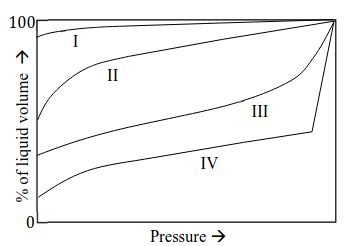
\includegraphics[width=0.4\columnwidth]{figs/fig6.png} 
   \caption*{}
  \label{fig:Q19}
\end{figure}

Which curve represents the Black Oil?

\hfill{\brak{\text{GATE PE 2022}}}

\begin{enumerate}
\begin{multicols}{4}
\item I
\item II
\item III
\item IV
\end{multicols}
\end{enumerate}

\item The dynamic mud inflow rate and mud outflow rate profiles are shown in the
following figure.

\begin{figure}[h!]
  \centering
  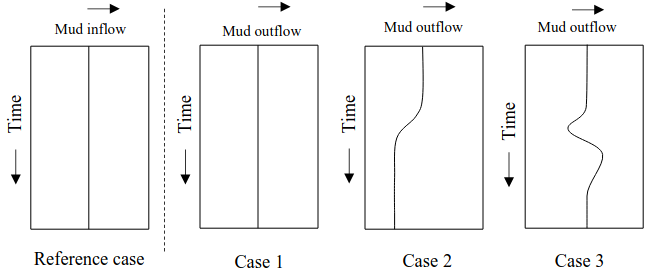
\includegraphics[width=0.8\columnwidth]{figs/fig7.png} 
   \caption*{}
  \label{fig:Q20}
\end{figure}

Identify the "Hole ballooning" and the "Lost circulation" phenomena.

\hfill{\brak{\text{GATE PE 2022}}}

\begin{enumerate}
\item Case 1 - Hole ballooning; Case 3 - Lost circulation
\item Case 2 - Lost circulation; Case 3 - Hole ballooning
\item Case 1 - Lost circulation; Case 2 - Hole ballooning
\item Case 2 - Hole ballooning; Case 3 - Lost circulation
\end{enumerate}

\item What is the maximum permissible limit of 'oil and grease' in discharged wastewater from a petroleum industry as per the guidelines of Central Pollution Control Board \brak{CPCB}, India?

\hfill{\brak{\text{GATE PE 2022}}}

\begin{enumerate}
\begin{multicols}{4}
\item 5 ppm
\item 10 ppm
\item 30 ppm
\item 50 ppm
\end{multicols}
\end{enumerate}

\pagebreak

\item The Timur chart for estimating the permeability is the plot between

\hfill{\brak{\text{GATE PE 2022}}}

\begin{enumerate}
\begin{multicols}{2}
\item Porosity and Water Saturation
\item True Resistivity and Water Saturation
\item Porosity and Irreducible Water Saturation
\item Porosity and True Resistivity
\end{multicols}
\end{enumerate}

\item The logging tool\brak{s} preferred for the measurement of formation resistivity in a well drilled with oil-based mud is/are

\hfill{\brak{\text{GATE PE 2022}}}

\begin{enumerate}
\begin{multicols}{2}
\item Dual Laterolog
\item Compensated Neutron Log
\item Compensated Density Log
\item Induction Log
\end{multicols}
\end{enumerate}

\item Which of the following properties of Matrix are CORRECT?

A =$\myvec{
1 & 0.5 & 0 \\
0.5 & 1 & 0.5 \\
0 & 0.5 & 1}$

\hfill{\brak{\text{GATE PE 2022}}}

\begin{enumerate}
\begin{multicols}{4}
\item Singular
\item Positive definite
\item Symmetric
\item Diagonal
\end{multicols}
\end{enumerate}

\item Simpson's one-third rule will give the exact value of the integral,  

\begin{align*}
I = \int_a^b \left( b_0 + b_1 x + b_2 x^2 + \dots + b_n x^n \right) dx
\end{align*}

\brak{\text{where $b_0, b_1, b_2, \dots, b_n$ are numeric constants}}, if the values of $n$ are

\hfill{\brak{\text{GATE PE 2022}}}

\begin{enumerate}
\begin{multicols}{4}
\item 1
\item 2
\item 3
\item 4
\end{multicols}
\end{enumerate}

\item Which of the following are NOT CORRECT during the operating cycle of a 'sucker rod pump'?

\hfill{\brak{\text{GATE PE 2022}}}

\begin{enumerate}
\item Standing valve is open during the upward stroke.
\item Standing valve is closed during the upward stroke.
\item Travelling valve is closed during the upward stroke.
\item Travelling valve is open during the upward stroke.
\end{enumerate}

\item Which of the following statements related to the 'enriched gas drive' are CORRECT?

\hfill{\brak{\text{GATE PE 2022}}}

\begin{enumerate}
\item The enriching components are transferred from the oil to the gas.
\item The enriched gas drive is an example of immiscible enhanced oil recovery.
\item A miscible zone is formed between the injected gas and the reservoir oil.
\item In enriched gas drive, the viscous fingering results in poor sweep efficiency.
\end{enumerate}

\item Select the CORRECT statements for the injection-production well pattern.

\hfill{\brak{\text{GATE PE 2022}}}

\begin{enumerate}
\item Inverted 5-spot drive includes four injectors at the corners and the producer at the centre.
\item Regular 7-spot drive includes six injectors at the corners and the producer at the centre.
\item Staggered-line drive involves staggered injectors and producers.
\item Crestal injection involves positioning of the wells along the periphery of the reservoir.
\end{enumerate}

\pagebreak

\item The flammable gas detector works on which of the following phenomena?

\hfill{\brak{\text{GATE PE 2022}}}

\begin{enumerate}
\begin{multicols}{4}
\item Catalytic
\item Paramagnetic
\item Electrochemical
\item Photoionisation
\end{multicols}
\end{enumerate}

\item A drilling mud with high gel strength is undesirable because it

\hfill{\brak{\text{GATE PE 2022}}}

\begin{enumerate}
\item retards the separation of cuttings and entrained gas at the surface.
\item leads to the lost circulation.
\item creates swabbing action beneath the bit while pulling the string.
\item leads to the hole ballooning.
\end{enumerate}

\item Which of the following Logging tool combinations are required to estimate the Hydrocarbon Initial in Place \brak{HCIP}?

\hfill{\brak{\text{GATE PE 2022}}}

\begin{enumerate}
\item Resistivity Log, Neutron Log and Gamma Ray Log
\item Sonic Log, Neutron Log and Gamma Ray Log
\item Resistivity Log, Density Log and Gamma Ray Log
\item Neutron Log, Density Log and Sonic Log
\end{enumerate}

\item A homogeneous sandstone reservoir is under a radial steady state flow. The wellbore radius is $0.1$ m. The formation near the wellbore is damaged up to $0.9$ m from the sand face. The permeability impairment results in $k/k_s = 5$, where $k$ is the permeability in the undamaged region and $k_s$ is that of the damaged region. The value of skin factor is \_\_\_\_\_\_\_\_\_ (rounded off to two decimal places).

\hfill{\brak{\text{GATE PE 2022}}}

\item A reservoir is producing oil at $7000$ stb/day with a producing gas to oil ratio \brak{GOR} of $2000$ scf/stb. At a certain point of time, the reservoir pressure is monitored and decided to be maintained at a constant pressure of $2500$ psi using water injection. The PVT properties estimated at $2500$ psi are:  

Bubble point pressure = $3000$ psi  
Oil formation volume factor = $1.2$ rb/stb  
Water formation volume factor = $1.0$ rb/stb  
Gas formation volume factor = $0.0012$ rb/scf  
Solution GOR = $300$ scf/stb  

The initial water injection rate \brak{stb/day} required to maintain oil production at $7000$ stb/day is \_\_\_\_\_\_\_\_\_ \brak{\text{rounded off to the nearest integer}}.

\hfill{\brak{\text{GATE PE 2022}}}

\item An oil well is drilled using an $8.5$-inch drill bit at a penetration rate of $30$ ft/hr. The rotary speed is $20$ rpm and the weight on the bit is $3500$ lb. The value of the 'd' exponent for the drilled section is \_\_\_\_\_\_\_\_\_ \brak{\text{rounded off to the nearest integer}}.

\hfill{\brak{\text{GATE PE 2022}}}

\item A vertical wellbore is drilled with a $12.25$-inch drill bit. While drilling, the bit could drill a total rock volume of $385$ ft$^3$ in $6.5$ hr. After drilling, the hole diameter throughout the depth is found to be $12.49$ inch. The average rate of penetration is \_\_\_\_\_\_\_\_\_ ft/hr \brak{\text{rounded off to the nearest integer}}.

\hfill{\brak{\text{GATE PE 2022}}}

\item A real gas is produced from a gas reservoir at a constant temperature of $30^\circ$C. The compressibility factor $\brak{Z}$ is observed to change with pressure $\brak{P}$ at a rate of $\dots$ . The difference in the compressibility of the real gas from the ideal gas at a given pressure $\brak{P}$ and temperature $\brak{T}$ is

\hfill{\brak{\text{GATE PE 2022}}}

\begin{enumerate}
\begin{multicols}{4}
\item $Z$
\item $2Z$
\item $\frac{Z}{2}$
\item $\frac{1}{2Z}$
\end{multicols}
\end{enumerate}

\pagebreak

\item A brine solution is being injected at a velocity $\brak{u}$ downward through a tubing of diameter $\brak{d}$ inclined at an angle of $\theta$ from vertical with gravitational acceleration $g$. Which ONE of the following options is CORRECT for the velocity $\brak{u}$ and the angle $\brak{\theta}$ such that the ratio of frictional pressure drop to the gravitational pressure drop is four times the Fanning friction factor?

\hfill{\brak{\text{GATE PE 2022}}}

\begin{enumerate}
\begin{multicols}{2}
\item $\sqrt{2gd}$ ; $30{\degree}$
\item $gd$ ; $30{\degree}$
\item $\sqrt{gd}$ ; $60{\degree}$
\item $\frac{1}{2}gd$ ; $30{\degree}$
\end{multicols}
\end{enumerate}

\item Which ONE of the following options is the CORRECT match of contaminants and their effluent treatment techniques?

\begin{tabular}{|c|c|}
\hline
\textbf{I.} Suspended solids & \textbf{P.} Ion exchange \\
\textbf{II.} Biodegradable organics & \textbf{Q.} Filtration \\
\textbf{III.} Heavy metals & \textbf{R.} Trickling filters \\
\textbf{IV.} Suspended oil and grease & \textbf{S.} Flocculation \\
\hline
\end{tabular}

\hfill{\brak{\text{GATE PE 2022}}}

\begin{enumerate}
\begin{multicols}{2}
\item I-P ; II-Q ; III-R ; IV-S
\item I-Q ; II-R ; III-P ; IV-S
\item I-Q ; II-S ; III-P ; IV-R
\item I-R ; II-S ; III-Q ; IV-P
\end{multicols}
\end{enumerate}

\item Capillary pressure $\brak{P_c}$ vs water saturation $\brak{S_w}$ curves for different sandstone reservoirs \brak{\text{I, II, III and IV}} are given in the following figure.

\begin{figure}[h!]
  \centering
  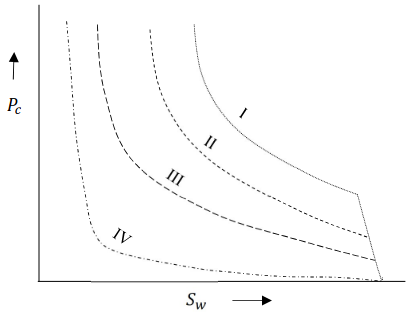
\includegraphics[width=0.4\columnwidth]{figs/fig8.png} 
   \caption*{}
  \label{fig:Q39}
\end{figure}

Which reservoir has the most uniform pore size distribution?

\hfill{\brak{\text{GATE PE 2022}}}

\begin{enumerate}
\begin{multicols}{4}
\item I
\item II
\item III
\item IV
\end{multicols}
\end{enumerate}

\pagebreak

\item Flow tests are conducted for oil well in reservoirs P, Q, R and S having different parameters as given in the following table. In all the four cases the wells are tested at $1200$ stb/day.

{\small
\begin{tabular}{|c|c|c|c|c|c|c|}
\hline
\textbf{Reservoir} & \textbf{Permeability} $\brak{\text{mD}}$ & \textbf{Porosity} $\brak{\%}$ & \textbf{Oil Viscosity} $\brak{\text{cP}}$ & \textbf{Total Compressibility} $\brak{\times 10^6 \ \text{psi}^{-1}}$ & \textbf{Wellbore Radius} $\brak{\text{ft}}$ & \textbf{Pay Zone Thickness} $\brak{\text{ft}}$ \\
\hline
P & 100 & 23 & 0.8 & 75 & 0.5 & 10 \\
Q & 50 & 21 & 1.1 & 70 & 0.4 & 12 \\
R & 150 & 25 & 0.9 & 80 & 0.3 & 15 \\
S & 170 & 28 & 1.0 & 90 & 0.6 & 20 \\
\hline
\end{tabular}
}

Identify the reservoir in which the pressure transient reaches earliest at a point $2000$ ft away from the wellbore.

\hfill{\brak{\text{GATE PE 2022}}}

\begin{enumerate}
\begin{multicols}{4}
\item P
\item Q
\item R
\item S
\end{multicols}
\end{enumerate}

\item Identify the CORRECT match for the flow regimes \brak{\text{Group 1}} with the corresponding slopes of the pressure derivative \brak{\text{Group 2}} used in the type curve analysis.

\begin{tabular}{|c|c|}
\hline
\textbf{Flow Regime \brak{\text{Group 1}}} & \textbf{Pressure Derivative Slope \brak{\text{Group 2}}} \\
\hline
I. Spherical flow & P. 1 \\
II. Linear flow & Q. $\frac{1}{4}$ \\
III. Bilinear flow & R. $-\frac{1}{2}$ \\
IV. Boundary dominated flow & S. $\frac{1}{2}$ \\
\hline
\end{tabular}

\hfill{\brak{\text{GATE PE 2022}}}

\begin{enumerate}
\begin{multicols}{2}
\item I-P; II-Q; III-R; IV-S
\item I-Q; II-S; III-R; IV-P
\item I-R; II-S; III-Q; IV-P
\item I-S; II-P; III-Q; IV-R
\end{multicols}
\end{enumerate}

\item The log data obtained for a particular well section are shown in the following figures.
Identify the CORRECT interpretations for different zones.

\begin{figure}[h!]
  \centering
  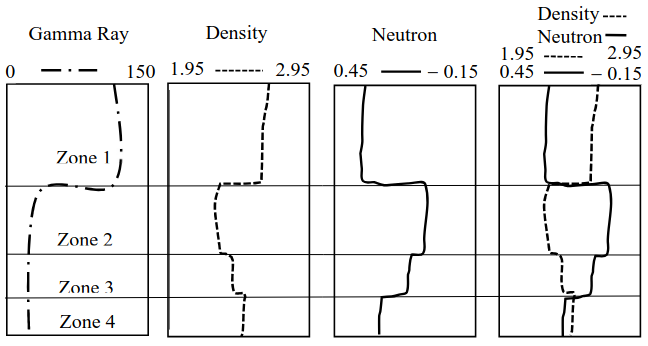
\includegraphics[width=0.6\columnwidth]{figs/fig9.png} 
   \caption*{}
  \label{fig:Q42}
\end{figure}

\hfill{\brak{\text{GATE PE 2022}}}

\begin{enumerate}
\item Zone 1 - shale; Zone 2 - clean sand with oil; Zone 3 - clean sand with gas; Zone 4 - clean sand with water
\item Zone 1 - clean sand with gas; Zone 2 - clean sand with oil; Zone 3 - clean sand with water; Zone 4 - shale
\item Zone 1 - shale; Zone 2 - clean sand with gas; Zone 3 - clean sand with oil; Zone 4 - clean sand with water
\item Zone 1 - clean sand with water; Zone 2 - clean sand with oil; Zone 3 - clean sand with gas; Zone 4 - shale
\end{enumerate}

\pagebreak

\item Well testing is to be conducted on the bounded sandstone reservoirs as shown in the following figures. All the reservoirs have the same drainage area, rock and fluid properties, and well bore conditions.

\begin{figure}[h!]
  \centering
  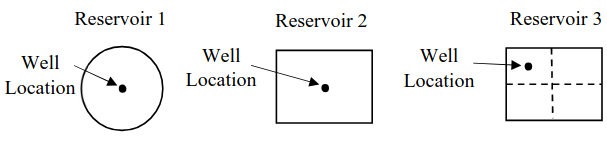
\includegraphics[width=0.8\columnwidth]{figs/fig10.png} 
   \caption*{}
  \label{fig:Q43}
\end{figure}

Which of the following statements are CORRECT for the given reservoirs?

\hfill{\brak{\text{GATE PE 2022}}}

\begin{enumerate}
\item Pseudo steady flow regime will develop first in Reservoir 1.
\item Infinite acting behavior will stop first in Reservoir 2.
\item Infinite acting behavior will sustain the longest in Reservoir 1.
\item Pressure depletion will be the fastest in Reservoir 3.
\end{enumerate}

\item An exploratory well is planned to be drilled in a basin that extends up to a depth of $5000$ m. The surface temperature is $30{\degree}$C. The geothermal gradient of the basin is $0.025{\degree}$C/m. Select the possible range\brak{\text{s}} of depth at which the potential oil bearing zones can be encountered.

\hfill{\brak{\text{GATE PE 2022}}}

\begin{enumerate}
\begin{multicols}{4}
\item 800 m to 950 m
\item 1500 m to 1650 m
\item 3100 m to 3150 m
\item 4550 m to 4600 m
\end{multicols}
\end{enumerate}

\item The following data are given for an oil well scheduled for a drawdown test.

\begin{tabular}{|l|l|}
\hline
Total compressibility & $20\times 10^{-6}\ \text{psi}^{-1}$ \\
Porosity & $15\%$ \\
Oil compressibility & $100\times 10^{-6}\ \text{psi}^{-1}$ \\
Wellbore radius & $0.25\ \text{ft}$ \\
Volume of fluid in the wellbore & $180\ \text{rb}$ \\
Oil viscosity & $2\ \text{cP}$ \\
Average oil density in the wellbore & $45\ \text{lb/ft}^3$ \\
Pay zone thickness & $50\ \text{ft}$ \\
Tubing outer diameter & $2\ \text{inch}$ \\
Skin factor & $0$ \\
Casing inner diameter & $7.675\ \text{inch}$ \\
Permeability & $30\ \text{mD}$ \\
\hline
\end{tabular}

If the well is tested at a constant rate, the 'Wellbore Storage Effect' would sustain for \_\_\_\_\_\_ hours \brak{\text{rounded off to two decimal places}}.

\hfill{\brak{\text{GATE PE 2022}}}

\pagebreak

\item During the core analysis, the following data are measured at laboratory and reservoir conditions.

\begin{tabular}{|l|c|c|}
\hline
Property & Laboratory condition & Reservoir condition \\
\hline
Interfacial tension \brak{\text{dynes/cm}} & 35 & 25 \\
Porosity \brak{\%} & 30 & 25 \\
Permeability \brak{\text{mD}} & 100 & 80 \\
Pore radius \brak{\text{$\mu$m}} & 22 & 18 \\
\hline
\end{tabular}

The capillary pressure at the laboratory condition is $50$ psi. The calculated capillary pressure using the Leverett J-function at the reservoir condition is \_\_\_\_\_ psi \brak{\text{rounded off to two decimal places}}.

\hfill{\brak{\text{GATE PE 2022}}}


\item The total oil production rate \brak{\text{measured at the bottom hole conditions}} from a volumetric reservoir is $200$ bbl/day \brak{\text{1 bbl = 5.615 ft$^3$}} at the flowing bottom hole pressure \brak{FBHP} of $3000$ psi. The reservoir has the following properties:

\begin{tabular}{|l|l|}
\hline
Pay zone thickness & $10$ ft \\
Porosity & $18\%$ \\
Total compressibility & $50 \times 10^{-6}\ \brak{\text{psi}^{-1}}$ \\
Permeability & $35$ mD \\
Wellbore radius & $0.25$ ft \\
Skin factor & $0$ \\
Drainage radius & $1000$ ft \\
\hline
\end{tabular}

Considering a radial flow under pseudo steady state, the bottom hole pressure after $180$ days is \_\_\_\_\_ psi \brak{\text{rounded off to two decimal places}}.

\hfill{\brak{\text{GATE PE 2022}}}


\item An incompressible fluid \brak{\text{density = 40 lb/ft$^3$}} flows at a steady state through a linear porous media with the following properties:

\begin{tabular}{|l|l|}
\hline
Length $\brak{L}$ & $1500$ ft \\
Permeability & $150$ mD \\
Height $\brak{H}$ & $15$ ft \\
Viscosity & $1.5$ cP \\
Width $\brak{W}$ & $30$ ft \\
Inlet pressure $\brak{P_1}$ & $1600$ psi \\
Porosity & $18\%$ \\
Outlet pressure $\brak{P_2}$ & $1590$ psi \\
\hline
\end{tabular}

\begin{figure}[h!]
  \centering
  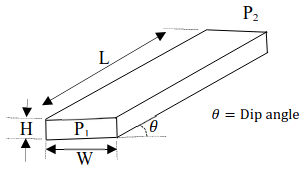
\includegraphics[width=0.4\columnwidth]{figs/fig11.png} 
   \caption*{}
  \label{fig:Q48}
\end{figure}


The absolute value of the difference between the actual fluid velocity \brak{\text{ft/day}} at $\theta = 0$ and $\theta = 10$ is \_\_\_\_\_ \brak{\text{rounded off to three decimal places}}.

\hfill{\brak{\text{GATE PE 2022}}}

\pagebreak

\item An oil well \brak{\text{wellbore radius = 0.5 inch}} in a heavy oil reservoir \brak{\text{drainage radius = 745 ft, oil viscosity = 500 cP}} is being operated at $200$ rb/day and $150$ psi under the radial steady state flow regime. A huff and puff steam injection is planned to reduce the oil viscosity to $35$ cP. The steam soaks into the reservoir up to a distance of $65$ ft from the centre of the wellbore. The new production rate at the downhole condition after the steam stimulation is \_\_\_\_\_ rb/day \brak{\text{rounded off to two decimal places}}.

\hfill{\brak{\text{GATE PE 2022}}}


\item If $Z$ is the standard normal variable having mean $0$ and standard deviation $1$, then the probability of occurrence of $Z$ in the range of $-3$ to $3$ is \_\_\_\_\_ \brak{\text{rounded off to three decimal places}}.

Given: 

\begin{align*}
\mathrm{erf}(z) \approx \tanh\!\left(\frac{167\,z + 11\,z^{3}}{148 + 109}\right)
\end{align*}

\hfill{\brak{\text{GATE PE 2022}}}

\item In a three dimensional $x y z$-space, if $\hat{v} = 3z\,\hat{i} + 2z\,\hat{j} + z\,\hat{k}$, and $\mathrm{curl}\,\hat{v} = \hat{v}_{a} = a\hat{i} + b\hat{j} + c\hat{k}$, then the value of $\brak{a+b+c}$ is \_\_\_\_\_ \brak{\text{in integer}}.

\hfill{\brak{\text{GATE PE 2022}}}


\item The local minimum value of the real function $f(x) = 3x^{4} - 22x^{3} + 36x^{2} - 20x$ is \_\_\_\_\_ \brak{\text{in integer}}.

\hfill{\brak{\text{GATE PE 2022}}}


\item Consider the following ordinary differential equation

\begin{align*}
\frac{dy}{dx} = x^{2}\,y
\end{align*}

The initial value is $y(0) = 1$ and the step-size is $0.1$. Solving this differential equation by Euler's first-order method, the value of $y(0.2)$ is \_\_\_\_\_ \brak{\text{rounded off to three decimal places}}.

\hfill{\brak{\text{GATE PE 2022}}}

\item In a horizontal circular pipe, liquid and gas are flowing concurrently at the same superficial velocity. However, the average velocity of the gas is greater than the average velocity of liquid. If the slip velocity is equal to the superficial velocity of each of the phases, the fractional liquid holdup is \_\_\_\_\_ \brak{\text{rounded off to two decimal places}}.

\hfill{\brak{\text{GATE PE 2022}}}

\item A $1$ kg-mol bottled gas consists of the following composition at $30{\degree}C$.

\begin{tabular}{|l|c|c|c|}
\hline
Component & n-Butane & Propane & Ethane \\
\hline
Composition \brak{\text{mol \%}} & $50$ & $45$ & $5$ \\
Vapour pressure \brak{\text{bar}} & $3$ & $10$ & $40$ \\
\hline
\end{tabular}

The equilibrium vapour composition of n-Butane in mol \% is \_\_\_\_\_ \brak{\text{rounded off to two decimal places}}.

\hfill{\brak{\text{GATE PE 2022}}}

\item A crude oil with a flowrate of $1000\ \text{kg/hr}$ is to be cooled using water in a double-pipe counter-flow heat exchanger from a temperature of $80{\degree}C$ to $40{\degree}C$. The water enters the exchanger at $20{\degree}C$ and leaves at $40{\degree}C$. The specific heat capacities of the oil and the water at constant pressure are $2\ \text{kJ kg}^{-1}\text{K}^{-1}$ and $4.2\ \text{kJ kg}^{-1}\text{K}^{-1}$, respectively. The overall heat transfer coefficient is $0.25\ \text{kW m}^{-2}\text{K}^{-1}$.  Neglecting the heat loss and using the log mean temperature difference $\brak{\text{LMTD}}$ method, the minimum heat exchanger area $\brak{\text{m}^2}$ required for the operation is \_\_\_\_\_ \brak{\text{rounded off to two decimal places}}.

\hfill{\brak{\text{GATE PE 2022}}}

\item In an oil reservoir undergoing water flooding, the areal and vertical sweep efficiencies are $0.75$ and $0.85$, respectively. The average water saturation behind the flood front is $0.63$ at breakthrough, and the initial water saturation is $0.17$. If the initial volume of in-situ oil at the start of water flooding is $3200\ \text{rb}$, the amount of oil produced during the water flooding is \_\_\_\_\_ rb \brak{\text{rounded off to two decimal places}}.

\hfill{\brak{\text{GATE PE 2022}}}

\pagebreak

\item The initial water saturation in an oil reservoir with a free gas cap is $30\%$. The initial gas saturation is $40\%$. At the end of water flooding, all the free gases are dissolved due to the elevated pressure and the oil formation volume factor reaches a value of $1.20\ \text{rb/stb}$. The final water saturation at the end of water flooding is $50\%$. If the two-phase formation volume factor at the initiation of the water flood is $2.3\ \text{rb/stb}$, the pore-to-pore displacement efficiency under the current reservoir condition is \_\_\_\_\_ \% \brak{\text{rounded off to one decimal place}}.

\hfill{\brak{\text{GATE PE 2022}}}


\item The station survey data during the directional drilling at two locations are given below.

\begin{tabular}{|l|c|c|}
\hline
Survey location & Depth \brak{\text{m}} & Inclination $\brak{\alpha}$ \brak{\text{(degree)}}; Azimuth $\brak{\beta}$ \brak{\text{(degree)}} \\
\hline
A & $4499$ & $\alpha = 14.8$, $\beta = \brak{\text{N19E}}$ \\
B & $4530$ & $\alpha = 13.5$, $\beta = \brak{\text{N10E}}$ \\
\hline
\end{tabular}

Dogleg angle $= \cos^{-1}\big[\cos\alpha_1\cos\alpha_2 + \sin\alpha_1\sin\alpha_2\cos(\beta_2-\beta_1)\big]$.

The calculated dogleg severity $\brak{\text{dogleg angle per 100 m of drilled section}}$ is \_\_\_\_\_ \brak{\text{rounded off to one decimal place}}.

\hfill{\brak{\text{GATE PE 2022}}}

\item A sandstone reservoir has the formation top at a depth of $3421$ ft from the surface as shown in the figure. The reservoir is logged with a modular dynamic tester $\brak{\text{MDT}}$. At a depth of $3425$ ft, the formation pressure is recorded as $1560$ psi and the sampled crude has a density of $35{\degree}\text{API}$.

\begin{figure}[h!]
  \centering
  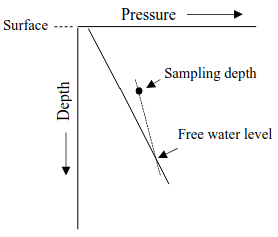
\includegraphics[width=0.4\columnwidth]{figs/fig12.png} 
   \caption*{}
  \label{fig:Q60}
\end{figure}

Considering a normal hydrostatic pressure gradient $\brak{\text{brine density} = 1.04\ \text{g/cc}}$ and a capillary displacement pressure of $1.2$ psi, the oil water contact $\brak{\text{OWC}}$ is found at a depth of \_\_\_\_\_ ft from the surface \brak{\text{rounded off to two decimal places}}.

\hfill{\brak{\text{GATE PE 2022}}}

\item The drill pipes and drill collars with a combined length of $2500\ \text{m}$ are held on the hook without rotation and mud flow. The specific gravity of the mud in the annulus is $1.5$ and that inside the drill string is $1.4$. The material density of the drill pipe and drill collar is $7850\ \text{kg/m}^3$. The specifications of drill pipes and drill collars are given below.

\begin{tabular}{|l|c|c|}
\hline
Specification & Drill pipe & Drill collar \\
\hline
Length \brak{\text{m}} & $2000$ & $500$ \\
Inside diameter \brak{\text{m}} & $0.106$ & $0.127$ \\
Outside diameter \brak{\text{m}} & $0.156$ & $0.406$ \\
Mass per unit length \brak{\text{kg/m}} & $30$ & $870$ \\
\hline
\end{tabular}

The overall weight acting on the hook is \_\_\_\_\_ kN \brak{\text{rounded off to two decimal places}}.

\hfill{\brak{\text{GATE PE 2022}}}

\pagebreak

\item A drilling rig is designed with $12$ lines strung between the crown block and the traveling block. The hoisting system has an output power of $650$ HP \brak{\text{1 HP = 33000 lb-ft/min}}. When the drill string is pulled up with a speed of $52.5$ ft/min, the tension in the fast line reads $46180$ lb. Assume that the rig utilizes all the available output power of drawworks and the drill string is pulled at a constant system efficiency. If the drill string is pulled at the same output power and the tension in the fast line is $35690$ lb, then the pullout speed of the drill string is \_\_\_\_\_ ft/min \brak{\text{rounded off to one decimal place}}.

\hfill{\brak{\text{GATE PE 2022}}}


\item In a sandstone reservoir, the density log reads $2.11\ \text{g/cc}$ and sonic log reads $90\ \mu\text{s/ft}$. The other parameters are given below:

\[
\begin{aligned}
\text{Matrix density } \brak{\rho_m} &= 2.68\ \text{g/cc} \\
\text{Fluid density } \brak{\rho_f} &= 1.0\ \text{g/cc} \\
\Delta t_m &= 54\ \mu\text{s/ft} \\
\Delta t_f &= 189\ \mu\text{s/ft}
\end{aligned}
\]

The calculated secondary porosity of the reservoir is \_\_\_\_\_ \% \brak{\text{rounded off to the nearest integer}}.

\hfill{\brak{\text{GATE PE 2022}}}


\item The Waxman--Smits equation to estimate water saturation for shaly sands is given as,

\begin{align*}
C_t = \phi^{m^*} S_w^{\,n^*}\,\brak{C_w + \dfrac{B\,Q_v}{S_w}}
\end{align*}

where $B$ is cation mobility $\brak{\text{m }\Omega^{-1}\ \text{meq}^{-1}\ \text{ml}^{-1}}$, and $Q_v$ is cation exchange capacity per pore volume $\brak{\text{meq ml}^{-1}}$.

\begin{tabular}{|l|c|}
\hline
Parameter & Value \\
\hline
Porosity $\brak{\phi}$ & $0.25$ \\
$B Q_v$ & $17.0\ \text{m }\Omega^{-1}$ \\
Cementation factor $\brak{m^*}$ & $2.0$ \\
Saturation exponent $\brak{n^*}$ & $2.0$ \\
Resistivity of water $\brak{R_w}$ & $0.05\ \Omega\ \text{m}$ \\
True resistivity (oil zone) $\brak{R_t}$ & $12\ \Omega\ \text{m}$ \\
\hline
\end{tabular}

As per the given dataset, the calculated water saturation $\brak{S_w}$ in the oil zone is \_\_\_\_\_ \% \brak{\text{rounded off to the nearest integer}}.

\hfill{\brak{\text{GATE PE 2022}}}

\item The hydrogen index $\brak{HI}$ of a potential source rock is $500$. If $400$ g of the same rock produces $6000$ mg of hydrocarbons during a thermal pyrolysis at the maximum temperature, the calculated total organic content $\brak{TOC}$ of the rock is \_\_\_\_\_ weight \% \brak{\text{rounded off to one decimal place}}.

\hfill{\brak{\text{GATE PE 2022}}}

\begin{center}
	{\LARGE \textbf{END OF THE QUESTION PAPER}}
\end{center}

\end{enumerate}

\end{document}
